\documentclass{article}
\usepackage[paperwidth=20cm, paperheight=21cm, margin=0.5cm]{geometry}
\usepackage{tikz}
\usetikzlibrary{arrows.meta, positioning, fit, backgrounds}
\usepackage[T1]{fontenc}
\usepackage{lmodern}
\pagestyle{empty}

\pgfdeclarelayer{background}
\pgfsetlayers{background,main}

% Colors
\definecolor{inputcol}{RGB}{224,242,254}
\definecolor{inputborder}{RGB}{14,116,144}
\definecolor{n1col}{RGB}{219,234,254}
\definecolor{n1border}{RGB}{30,58,138}
\definecolor{n2col}{RGB}{220,252,231}
\definecolor{n2border}{RGB}{22,101,52}
\definecolor{n3col}{RGB}{254,243,199}
\definecolor{n3border}{RGB}{146,64,14}
\definecolor{extcol}{RGB}{243,232,255}
\definecolor{extborder}{RGB}{107,33,168}
\definecolor{outcol}{RGB}{255,241,242}
\definecolor{outborder}{RGB}{159,18,57}
\definecolor{lgbg}{RGB}{248,250,252}
\definecolor{lgborder}{RGB}{100,116,139}
\definecolor{arrowcol}{RGB}{51,65,85}

\tikzset{
  main/.style={rectangle, rounded corners=5pt,
    minimum width=7cm, minimum height=1.2cm,
    align=center, draw, line width=1.1pt},
  ext/.style={rectangle, rounded corners=5pt,
    minimum width=4.2cm, minimum height=1.0cm,
    align=center, draw, line width=0.9pt},
  arr/.style={-{Stealth[length=6pt]}, line width=1.4pt, color=arrowcol},
  darr/.style={-{Stealth[length=5pt]}, line width=0.9pt, dashed, color=extborder},
}

\begin{document}
\centering
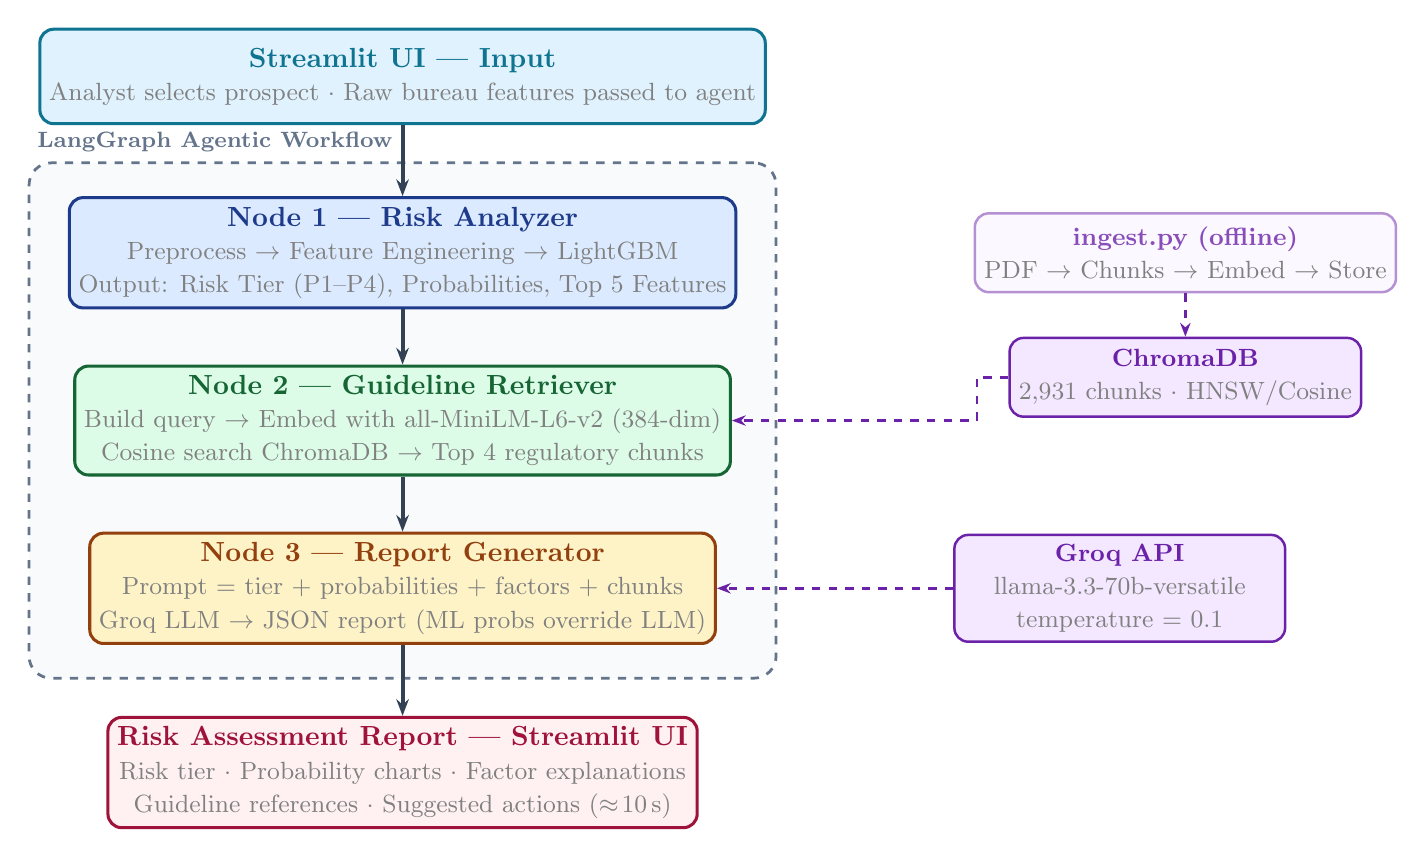
\begin{tikzpicture}[node distance=0.75cm and 3.2cm]

  \node[main, fill=inputcol, draw=inputborder] (input) {
    \textbf{\color{inputborder}Streamlit UI --- Input}\\
    {\small\color{gray}Analyst selects prospect $\cdot$ Raw bureau features passed to agent}
  };

  \node[main, fill=n1col, draw=n1border, below=0.9cm of input] (n1) {
    \textbf{\color{n1border}Node 1 --- Risk Analyzer}\\
    {\small\color{gray}Preprocess $\to$ Feature Engineering $\to$ LightGBM}\\
    {\small\color{gray}Output: Risk Tier (P1--P4), Probabilities, Top 5 Features}
  };

  \node[main, fill=n2col, draw=n2border, below=0.7cm of n1] (n2) {
    \textbf{\color{n2border}Node 2 --- Guideline Retriever}\\
    {\small\color{gray}Build query $\to$ Embed with all-MiniLM-L6-v2 (384-dim)}\\
    {\small\color{gray}Cosine search ChromaDB $\to$ Top 4 regulatory chunks}
  };

  \node[main, fill=n3col, draw=n3border, below=0.7cm of n2] (n3) {
    \textbf{\color{n3border}Node 3 --- Report Generator}\\
    {\small\color{gray}Prompt = tier + probabilities + factors + chunks}\\
    {\small\color{gray}Groq LLM $\to$ JSON report (ML probs override LLM)}
  };

  \node[main, fill=outcol, draw=outborder, below=0.9cm of n3] (output) {
    \textbf{\color{outborder}Risk Assessment Report --- Streamlit UI}\\
    {\small\color{gray}Risk tier $\cdot$ Probability charts $\cdot$ Factor explanations}\\
    {\small\color{gray}Guideline references $\cdot$ Suggested actions $(\approx\!10\,\mathrm{s})$}
  };

  % LangGraph box in background layer
  \begin{pgfonlayer}{background}
    \node[draw=lgborder, fill=lgbg, rounded corners=8pt,
          line width=1pt, dashed,
          inner xsep=14pt, inner ysep=12pt,
          fit=(n1)(n2)(n3)
         ] (lgbox) {};
    \node[font=\footnotesize\bfseries\color{lgborder},
          anchor=south west] at (lgbox.north west) {LangGraph Agentic Workflow};
  \end{pgfonlayer}

  % External: ingest.py
  \node[ext, fill=extcol!30, draw=extborder!50,
        right=3.0cm of n1] (ingest) {
    \textbf{\small\color{extborder!80}ingest.py (offline)}\\
    {\small\color{gray}PDF $\to$ Chunks $\to$ Embed $\to$ Store}
  };

  % External: ChromaDB
  \node[ext, fill=extcol, draw=extborder,
        below=0.55cm of ingest] (chroma) {
    \textbf{\small\color{extborder}ChromaDB}\\
    {\small\color{gray}2{,}931 chunks $\cdot$ HNSW/Cosine}
  };

  % External: Groq
  \node[ext, fill=extcol, draw=extborder,
        right=3.0cm of n3] (groq) {
    \textbf{\small\color{extborder}Groq API}\\
    {\small\color{gray}llama-3.3-70b-versatile}\\
    {\small\color{gray}temperature = 0.1}
  };

  % Main flow
  \draw[arr] (input) -- (n1);
  \draw[arr] (n1)    -- (n2);
  \draw[arr] (n2)    -- (n3);
  \draw[arr] (n3)    -- (output);

  % External connections
  \draw[darr] (ingest) -- (chroma);
  \draw[darr] (chroma.west) -- ++(-0.4,0) |- (n2.east);
  \draw[darr] (groq.west)   -- (n3.east);

\end{tikzpicture}
\end{document}
